\section{Analysis and Design} \label{sec:Design}

Seeing that this is a system dealing with finance, it would make sense to treat
the categories as if they were the accounts. And, in order to make sure to
imbue this system with knowledge acquired by more experienced programmers, it
makes sense to make use of patterns.

% maybe move to appendix
It is also useful at this point to make a distinction between the types of
classes used to model the domain between three possible kinds: the first are
the classes which model the interaction between the system and its actors --
these are called \emph{boundary classes}; the second kind are those classes
which model information and/or behaviour or some concept or phenomenon -- these
will be called \emph{entity classes}; and lastly, there are those classes which
model transactions, coordination, control and sequencing of other objects --
which are known as \emph{control classes} (Jacobson et al., 1999,
\cite[cited][pp.~198-201]{bennett2010object}).

The first analysis patterns which seem appropriate are the \emph{Account}
pattern, used to create the \emph{Category} entity class, and the
\emph{Quantity} pattern for the \emph{Amount} entity class
(\cite[][Sections~6.1~\&~3.1]{fowler1997analysis}):
\begin{figure}[ht!]
  \begin{center}
    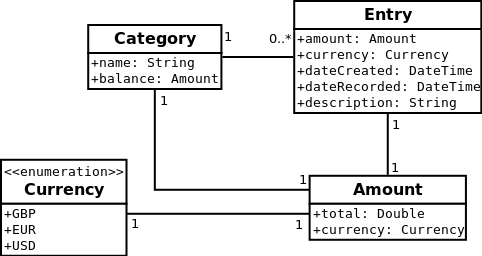
\includegraphics[width=11cm]{./contents/img/Class_Diagram_-_Categories_and_Amount.png}
  \end{center}
\end{figure}
\FloatBarrier

As implied by the diagram above, the \emph{Category} class will be associated
with instances of the \emph{Entry} class, and will keep track of the balance
made up of the sum of \emph{Amount}'s of each entry. This is done so that the
only way to change the total of a category is by adding positive or negative
entries to it -- for example, to indicate a credit to a category, a negative
entry can be added to it.

The next step is to provide a way for these entries to be added to categories.
For this to happen, there needs to be a constraint in to ensure that double
entry happens every time a change needs to be made to a category. One of the
ways to achieve this is to apply the \emph{Transaction} pattern
(\cite[][Section~6.2]{fowler1997analysis}):
\begin{figure}[ht!]
  \begin{center}
    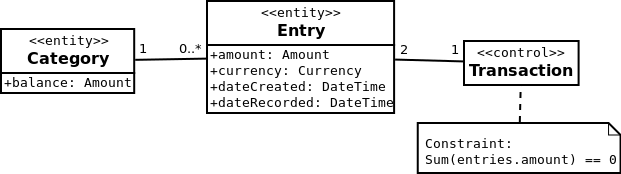
\includegraphics[width=14cm]{./contents/img/Class_Diagram_-_Transaction.png}121200
  \end{center}
\end{figure}
\FloatBarrier

